\section*{Введение}
\addcontentsline{toc}{section}{Введение}

Астрофизический $r$-процесс, или процесс быстрого нейтронного захвата, является механизмом нуклеосинтеза, в ходе которого исходное ядро поглощает большое число нейтронов и, оказавшись в области нейтронного избытка, испытывает слабые распады. В результате масса ядра увеличивается за счет поглощенных нейтронов, а $\beta^-$-распады приводят к образованию химического элемента с большим зарядовым числом. В $r$-процессе скорости нейтронного захвата на порядки превышают скорости $\beta^-$-распадов, что обеспечивает стремительный набор массы и значительное смещение в область нейтронного избытка. Для достижения необходимой интенсивности поглощения нейтронов требуется высокая плотность их потока, около 150 нейтронов на одно зародышевое ядро, и температуры вещества свыше 1~ГК. Такие экстремальные условия могут реализовавываться в катастрофических астрофизических явлениях: взрывах сверхновых, слияниях нейтронных звезд или нейтронной звезды и черной дыры. 

По современным представлениям, именно $r$-процесс обеспечивает возникновение основной массы ядер химических элементов тяжелее железа во Вселенной. Синтез более легких ядер обеспечивается термоядерным горением звездного вещества, но, как известно, им невозможно объяснить синтез ядер за так называемым <<железным пиком>>, максимумом зависимости удельной энергии связи от массового числа. Процесс медленного нейтронного захвата, $s$-процесс, отличающийся от $r$-процесса значительно меньшей интенсивностью поглощения нейтронов и, соответственно, характерными временами порядка сотен лет, требует не столь исключительных астрофизических условий и позволяет объяснить возникновение стабильных изотопов вплоть до висмута. Однако $s$-процесс не может преодолеть область

\begin{figure}
  \centering
  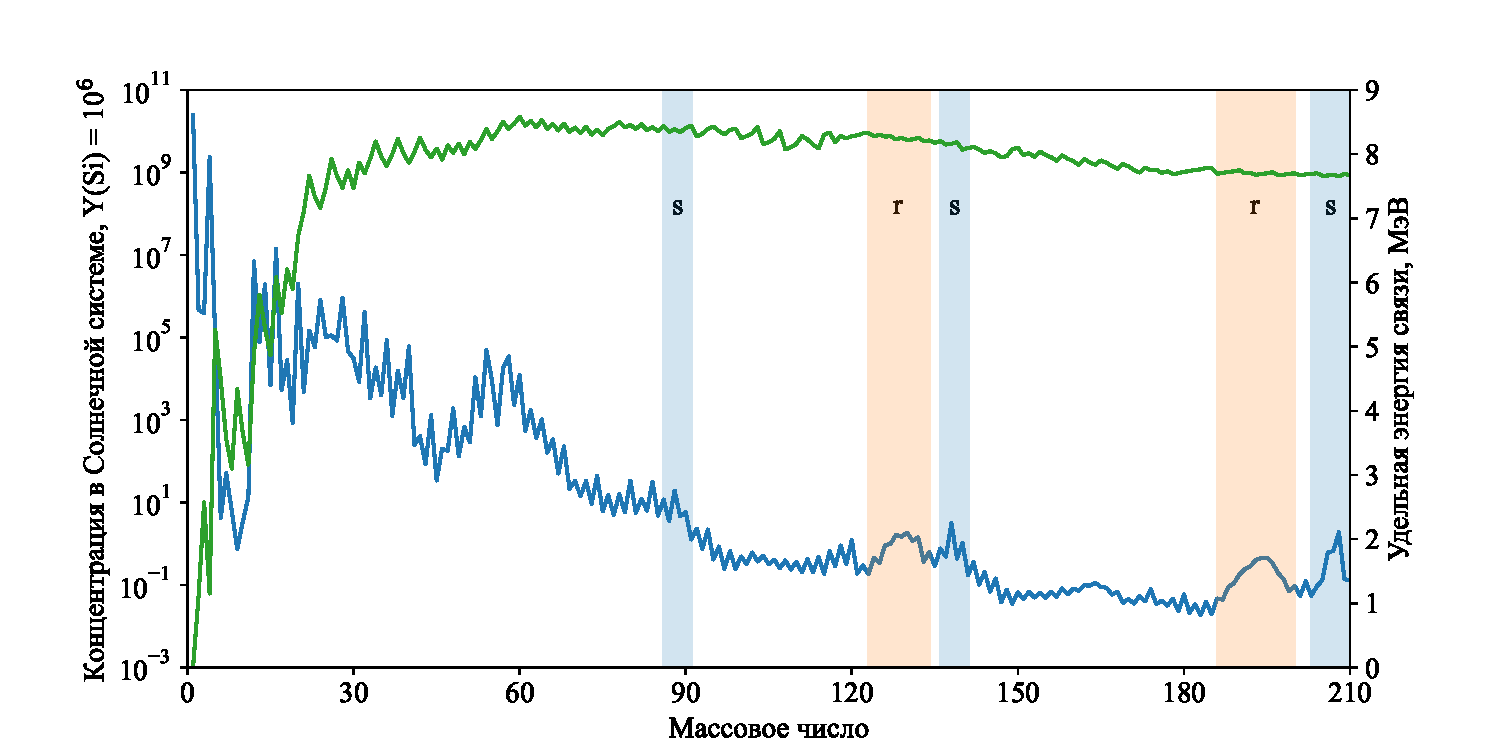
\includegraphics[width=0.8\textwidth]{pics/lodders_vs_ame.pdf}
  \caption{Удельная энергия связи (оранжевым, максимальное значение при данном $A$)~\cite{huang2021} и распространенности ядер в Солнечной системе (синим)~\cite{lodders2003}.}
  \label{img:lodders_vs_ame}
\end{figure}




Основным методом исследования $r$-процесса и эволюции астрофизических ядерных систем в целом является математическое моделирование. Для получения надежных результатов симуляции необходимо достоверно знать ряд входных параметров, таких как состав звездного вещества, его температуры и плотности, а также сечения ядерных реакций, протекающих в звездах. На данный момент эти величины известны в основном из теоретических моделей, астрофизических и ядерных, что вызывает существенные неопределенности входных данных.


